% !TEX TS-program = pdflatex
% !TEX encoding = UTF-8 Unicode

% This is a simple template for a LaTeX document using the "article" class.
% See "book", "report", "letter" for other types of document.

\documentclass[11pt]{article} % use larger type; default would be 10pt

\usepackage[utf8]{inputenc} % set input encoding (not needed with XeLaTeX)
\usepackage{graphicx}
\graphicspath{{images/}}
\usepackage{gensymb}
\usepackage[hidelinks]{hyperref}

%%% Examples of Article customizations
% These packages are optional, depending whether you want the features they provide.
% See the LaTeX Companion or other references for full information.

%%% PAGE DIMENSIONS
\usepackage{geometry} % to change the page dimensions
\geometry{a4paper} % or letterpaper (US) or a5paper or....
% \geometry{margin=2in} % for example, change the margins to 2 inches all round
% \geometry{landscape} % set up the page for landscape
%   read geometry.pdf for detailed page layout information

\usepackage{graphicx} % support the \includegraphics command and options

% \usepackage[parfill]{parskip} % Activate to begin paragraphs with an empty line rather than an indent

%%% PACKAGES
\usepackage{booktabs} % for much better looking tables
\usepackage{array} % for better arrays (eg matrices) in maths
\usepackage{paralist} % very flexible & customisable lists (eg. enumerate/itemize, etc.)
\usepackage{verbatim} % adds environment for commenting out blocks of text & for better verbatim
\usepackage{subfig} % make it possible to include more than one captioned figure/table in a single float
\usepackage{amsmath}
% These packages are all incorporated in the memoir class to one degree or another...

%%% HEADERS & FOOTERS
\usepackage{fancyhdr} % This should be set AFTER setting up the page geometry
\pagestyle{fancy} % options: empty , plain , fancy
\renewcommand{\headrulewidth}{0pt} % customise the layout...
\lhead{}\chead{}\rhead{}
\lfoot{}\cfoot{\thepage}\rfoot{}

%%% SECTION TITLE APPEARANCE
\usepackage{sectsty}
\allsectionsfont{\sffamily\mdseries\upshape} % (See the fntguide.pdf for font help)
% (This matches ConTeXt defaults)
\setcounter{secnumdepth}{5}
%%% ToC (table of contents) APPEARANCE
\usepackage[nottoc,notlof,notlot]{tocbibind} % Put the bibliography in the ToC
\usepackage[titles,subfigure]{tocloft} % Alter the style of the Table of Contents
\renewcommand{\cftsecfont}{\rmfamily\mdseries\upshape}
\renewcommand{\cftsecpagefont}{\rmfamily\mdseries\upshape} % No bold!

%%% END Article customizations

%%% The "real" document content comes below...

\title{Face Tracking for Optimized Bitrate Control in Low Delay Video Encoding}
\author{Chethan Ningaraju}
%\date{} % Activate to display a given date or no date (if empty),
         % otherwise the current date is printed 

\begin{document}
\maketitle
\clearpage
\tableofcontents
\clearpage
%%%
%%%%INTRODUCTION
%%%%
\section{Introduction}
	In recent years, there is increasing demand for high-quality video conferencing solutions. Due to availability of high-speed and low-delay internet, video conferencing has proved to be an efficient alternative to face-to-face meeting. Video telephony has grown into a multi-billion dollar industry and has huge commercial significance. To address this growing need there has been constant improvement in  low-delay video coding techniques along with better techniques to ensure low-delay transmission reliability at the network level. The tremendous increase in smartphone usage has led to increase in video telephony over cellular networks whose bandwidth is highly constrained. Therefore, it is very important to develop methods of delivering high quality video with less bandwidth requirement. 

The most commonly used video coding standards like H.264/AVC have been designed to exploit the spatial and temporal redundancy in the input video stream to achieve high data compression. The techniques of spatial and temporal prediction forms the core principle of these video coding standards. However, after encoding the video the perceptual redundancies still remains, since human attention does not focus on the whole scene but only a small region of fixation called region-of-interest (ROI) \cite{Perception-model-of-face}. Therefore, reducing the perceptual redundancy gives a new dimension towards achieving lower bit-rate at acceptable perceptual quality.

The goal of this work is to identify the salient region of a frame, which is the face of the participant in a video conference. Since the attention of the viewer is mostly focused on the face of the other participants during a video conference call, improving the quality of the face region (ROI) can improve the overall perceptual quality. In this work, we assume ideal capture conditions and use the results of the face tracking directly as side information for the H264/AVC encoder's bitrate control. This work explores the methods of region of interest(ROI) based encoding to exploit the available bandwidth to encode regions that are of high importance to perceptual quality with higher quality. Face region in the input stream is allocated an above-average bit-count to yield a better visual quality than the background regions. It is also the aim of this work to develop and extensively evaluate the strategy of uneven bit-allocation and also to identify its limitations.

\subsection{ROI-based Coding}

In conventional video coding, all regions of a frame are considered equally important to the viewer. It is assumed that all regions contribute equally to the perceptual quality. However, the study of Human Visual System (HVS) shows that human eyes can only focus on one area in a frame at any given point in time which is called region of interest. For example, it has been found out in \cite{human-vision-proof-NSI} that humans normally perceive clearly a small region of 2–5\degree of the visual angle.

In video coding, the compression gains from spatial and temporal prediction is reaching saturation level. Further compression from these techniques demand exponential growth in computational capabilities. Therefore, perceptual coding can provide an efficient solution towards lower bitrate video coding. Some of the commonly used video codecs use the fact that high frequency components are less important to the human visual system and perform preferential coding based on spatial frequency. The higher frequency components which are not so important to the perceptual quality are encoded with higher QP. However, such preferential coding does not take into account the region of interest to the viewer in the frame to be encoded. All high frequency components are coded with higher quantization irrespective of the region belonging to ROI. 

The ROI-based coding is not a common practice in video coding because it is very hard to automatically detect important regions in generic contents that contribute the most to the perceptual quality. There are many ways of detecting region of interest, most of which are application specific. The most common approach is usage of difference image based moving object detector. In these systems any moving object is considered as ROI. A typical use-case for such a system is video surveillance. In addition to difference image based motion detection, global motion estimation is used in ROI detection \cite{ROI-aerial-surveillance} in applications like aerial surveillance.

In generic video content region of interest constantly keeps changing depending on the context. For instance, in a movie, the ROI can depend on context of the scene. Developing generic techniques for detection of ROI in such videos is very difficult. There have been attempts to use eye tracker to record the foveation points of a human observer on the receiver which was used to apply foveation filter in video coding of the sender. An advancement over such approach is proposed in \cite{foveated-rate-control} which optimizes rate control to maximize foveal visual quality metric. These generic ROI detectors are very hard to implement due to uncommon availability of eye tracking mechanism at the receiver. 

The region of interest in the video conferencing scenario is going to be the face region predominantly. Due to recent improvements in face detection algorithms it is possible to detect the face with good accuracy. The study in \cite{HighQualityROICodingForVideoConferencing} shows how boosting quality of the face regions can improve the overall perceived quality of the video. This work aims to study possible ways of improving perceptual quality of the video by detecting face region and coding it with higher quality than rest of the frame.

The knowledge of region of interest in input video can be used for many other purpose in addition to its use in video coding to improving perceptual quality. For instance, ROI information can be used in developing techniques for smart thumbnail display in group video conferencing solutions. In group video conferencing, an active person is detected based on the source of voice and is displayed on the main screen and other participants are displayed on the smaller windows with down-scaling of the entire video. If the face coordinates of the participant is transmitted along with the bit-stream as meta-data, a cropped version of video can be displayed to show only the face in thumbnail display. This can improve overall user-experience.

\subsection{Bitrate Control} \label{Intro:Bitrate-Control}
	The bitrate control module is responsible for controlling the bit-consumption of the encoder to guarantee smooth playback. Bitrate control is not video coding standard specific and operates independent of any chosen video coding standard. There are various flavors of bitrate control like Constant Bitrate (CBR), Variable Bitrate (VBR) and Average Bitrate (ABR). In this work, CBR type of bitrate control is considered since it is most commonly used in video conferencing and other real-time streaming applications. 
\begin{figure}[h]
    \centering
    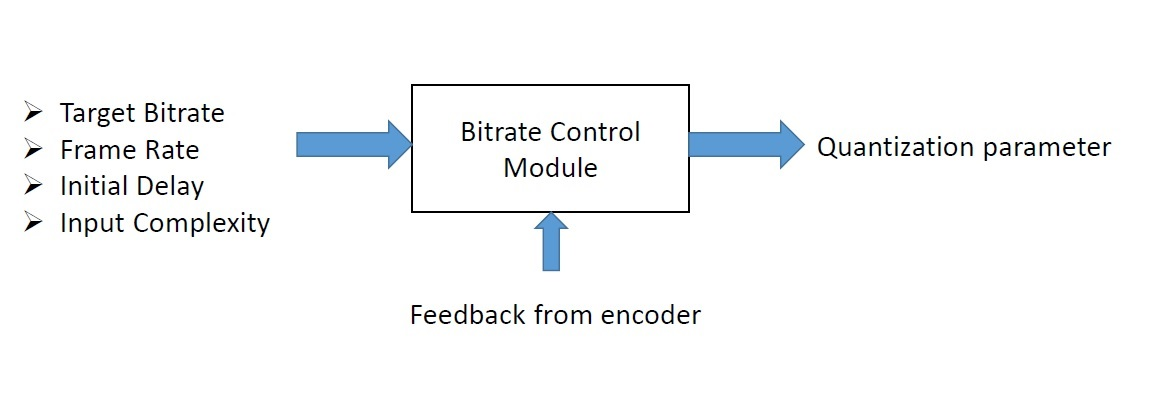
\includegraphics[scale=0.5]{RC_block}
    \caption{Bitrate Control Module Functionality}
    \label{fig:Bitrate Control Module Functionality}
\end{figure} 

\begin{figure}[h]
    \centering
    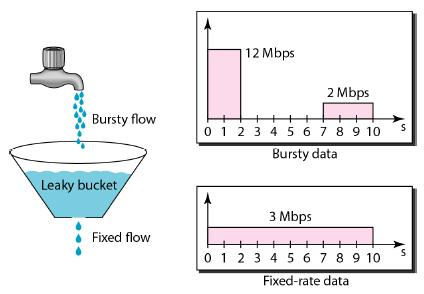
\includegraphics[scale=0.5]{general/Leaky_bucket}
    \caption{Leaky Bucket Model}
    \label{fig-Leaky-Bucket-Model}
\end{figure} 	
	Figure \ref{fig:Bitrate Control Module Functionality} illustrates the functionality of the bitrate control module. The main purpose of the bitrate control module is to ensure smooth playback of the encoded video under given bandwidth and delay constraints. It estimates the video bitrate based on the available network bandwidth, ensures the coded bitstream can be transmitted successfully and makes full use of the limited bandwidth \cite{InTech-Rate-control-in-video-coding}. It achieves this by controlling the quantization parameter (QP) used during the encoding. The quantization parameter is computed considering the input bitrate, framerate, input complexity (spatial and temporal activity) and acceptable delay of the system. The module also takes the feedback from the encoder regularly to make better QP decision.  The feedback from the encoder gives information about the content of the video and helps the bitrate control to compute right QP for a given bit-budget.
	
	The functionality of the Bitrate control module can be illustrated with the help of leaky-bucket model \cite{InTech-Rate-control-in-video-coding}. The output data-rate of a video encoder varies depending on the input complexity of the video (motion in the frame). It also depends on the picture type of the encoded frame. A frame can be encoded with spatial prediction (Key/I-frames), single direction temporal prediction (P-frames) and Bi-direction temporal prediction (B-frames). The key/I-frames consume a lot of bits compared to inter pictures (P-frames and B-frames). In a video streaming scenario considering a constant bitrate channel, the throughput is maximum when data-rate is constant and equal to the available bandwidth. Therefore, the output data of the encoder is smoothened using a theoretical buffer called Video Buffer Verifier (VBV). The VBV buffer is a virtual buffer modeled by the bitrate control module to ensure that video stream can be correctly buffered, and played back at the decoder end. This is equivalent to a leaky-bucket model as shown in Figure \ref{fig-Leaky-Bucket-Model} \cite{Leaky-bucket-NSI}, where the output of the encoder with variable rate (bursty output) is stored in a buffer (leaky bucket) which is draining at a constant rate.  Any underflow or overflow of this buffer causes glitch in the video streaming. To ensure that there is no VBV buffer overflow or underflow, encoder's quantization parameter is adapted on a macroblock level so that the maximum allowed bit-count for an encoded frame is not exceeded.

 A typical bitrate control allocates bits at every macroblock and adjusts the QP. In a simple approach one would try to distribute the bitrate evenly across all macroblocks in the frame. Since load efficiency is of high importance it is not advisable to do multi-pass encoding for optimal bitrate allocation. Therefore, over-allocation in one macroblock has to be compensated by under-allocation (using a higher QP) for neighboring macroblocks, regardless of the image content. However, a more intelligent allocation strategy should take the image content into account. Thus parts of the image with higher importance (ROI) should be given a higher share of the overall bit-count which results in higher visual quality. Background regions would get a lower proportion of the bit-count.

%% Section to throw light on other works in same field
\section{Related Work}

The concept of region of interest based encoding has been around for a while. The different approaches of using ROI information to improve perceptual quality can be broadly classified into following categories based on which stage of processing the ROI information is used.
\begin{itemize}  
\item Preprocessing - Blurring
\item Video encoding - During RDO, bitrate control
\end{itemize}
The input video stream can be directly altered based on the ROI information. Many pre-processing approaches are also used to directly reduce unimportant information by applying a non-uniform distortion filter in a scene. For instance, the image is divided into foreground (ROI) and background (non-ROI) and the non-ROI parts are blurred in \cite{ROI-background-blurring} to save bits during encoding. The work in \cite{pre-postprocessig-ROI-codec-independent} is an example for codec independent ROI encoding. It can work with any codec and arbitrary ROI detector. In this approach input video stream is modified only to contain relevant information. The non-ROI pixels are replaced such that these regions can be very efficiently compressed by the encoder. The non-ROI macroblocks are either replaced by corresponding block from the previous frame or a black block. The non-ROI regions are reconstructed with post-processing assuming zero motion vector. This approach is used in scenarios where non-ROI regions are mostly discarded completely at the receiver end.

In video encoding, multiple approaches exist to preferentially code ROI regions with higher quality at the cost of non-ROI regions. The ROI information can be directly used in rate-distortion optimization (RDO) during video encoding to alter the quality of ROI region. One such approach is presented in \cite{ROI-rate-control-H264} in which non-ROI macroblocks are encoded only using AMC-based modes (Active MB Concealment). The non-ROI macroblocks are encoded with only motion vector but no residual information. This creates a bias to choose larger distortion for non-ROI blocks to save bits during Lagrangian optimization.

A more common way of ROI encoding is by altering the rate control module to allocate higher bits to ROI regions. The work in \cite{ROI-bit-allocation-h264} proposes a bit-allocation and rate control scheme for enhancing regional perceptual quality using SSIM as the quality metric for distortion-quantization modeling. Statistical analysis is adopted to obtain the relation between SSIM of reconstructed MBs and corresponding QP (from 20 to 51 in this paper) after standard video coding.

The ROI-based encoding specific to video conferencing is proposed in \cite{ROI-MV-based-face-tracking} for H.263. This work proposes an algorithm to track face using motion-vector information. Once ROI is detected, it proposes modification of bit-allocation for both CBR and VBR mode of rate control. The QP for these blocks is predicted from the rate modeling of ROI and non-ROI blocks. The work described in \cite{Perception-model-of-face} goes a step further in face detection based ROI encoding schemes by enhancing finer facial feature to improve the perceptual quality in high-resolution HEVC encoding. In this approach, different weights are assigned to the background, face, eyes, mouth and nose regions which are in-turn used to alter quality by ROI-based adaptive CTU (Coding Tree Unit) partition structure for HEVC.

Most of the previous work concerned with modification of rate control to achieve better quality in ROI macroblocks deals with altering bit-allocation module. This work proposes ways of achieving ROI encoding in rate control modules that do not have explicit bit-allocation at the macroblock level. The previous works mentioned above proposes effective methods to create the quality difference between ROI and non-ROI. They do not throw sufficient light on determining optimal quality difference to achieve best perceptual quality. The goal of this work is also to come up with a guideline to determine optimal quality difference to achieve best perceptual quality.

%%section for detailed overview of bitrate control	
\section{Overview of Bitrate Control Module} \label{used-bitrate-control-overview}
This section gives an overview of the low-delay bitrate control module used in this work. The need for extremely low end-to-end delay in video telephony puts additional constraints on video coding which results in compromise of video quality. During the low-delay video encoding, tools like bi-directional prediction (B-frames) are disabled. The usage of B-frames needs buffering of at least one frame. This adds on to overall latency of the system which is highly undesirable in video conferencing. The tolerable delay in video encoding is a direct measure of Video Buffer Verifier (VBV) buffer size. When the size of the VBV buffer is very low (due to low delay), there is less room to accommodate the variation in bitrate of the encoder. This implies that there can be minimum variation in the size of a frame irrespective of the content. Any wrong prediction of QP by the bitrate control module can have bad impact since there is no additional time available to re-encode the content with corrected QP. 
 
 The bitrate control module used in this work is a modified version of \cite{JVTF086}.  The bitrate control does a frame level bit-allocation based on fullness of the VBV buffer, followed by adapting QP at the macroblock level. The functionality of the bitrate control module can be divided into two parts:
\begin{itemize}  
\item Bit Allocation
\item QP Prediction
\end{itemize}

\subsection{Bit Allocation}

The low-delay encoding mode does not favor usage of key frames at regular intervals and B-frames. Therefore, in steady state only P-frames are used in encoding video conferencing content. This makes frame level bit-allocation simpler since there is no need to consider relative complexity between different types of frames during frame level bit-allocation. The key-frame at the beginning is handled using special cases.  

As depicted in Figure \ref{fig:Bitrate Control Module Functionality}, one of the inputs for bitrate control module is a delay/latency parameter (L). This is defined as the maximum permissible delay allowed between the encoder and the decoder assuming zero transmission delay. In other words, the delay parameter is the maximum allowed time for any encoded frame to be transmitted completely through a constant bandwidth channel of per-defined bitrate. In this work, delay parameter (L) is configured as,
\begin{equation} 
	L_0 = 165 ms \text{	and	} L = \frac{1.5 * 1000}{framerate}.
\end{equation}
Initially a delay of $L_0 = 165ms$ is allowed for the key-frame. This allows, allocation of higher than average bits for the key-frame. However, the delay parameter (L) for P frames in steady state is only 1.5 times the frame sampling delay. For instance, if the input video is sampled at 30 frames/sec, then the time interval between two consecutive frame is 33ms (frame sampling delay), the permissible delay(L) for frames in steady state is approximately 49ms. The usage of different delay values for first key frame and steady state P-frames is handled by changing the delay value gradually. The large key-frame at the beginning results in huge delay (165ms), this delay is gradually reduced by using less than average bit-count for subsequent few frames (half of average bit-count per frame). Once the over-consumption of first-key frame is compensated, the steady state delay of $49ms$ is maintained for rest of the sequence.

It should be noted that the initial delay in the system can only be reduced by displaying the initial few P-frames at shorter intervals than the time interval in which they were captured. This results in momentary increase in playback speed. In practical implementation, usage of above average bit-count for I-frame results in few dropped frames subsequently even if I-frame over-consumes marginally. All the above artifacts are considered as an acceptable trade-off to achieve good initial spatial quality by allocating huge amount of bits to the first key-frame.

The bit-allocation module uses VBV buffer fullness and delay parameter (L) to compute the bits allocated for the current frame to be encoded. The VBV buffer fullness before encoding $nth$ frame ($d_0^{n}$) is calculated based on the size of the previously encoded $(n-1)th$ frame in bits ($FrameSize_{n-1}$) as follows,

$$ d_0^{n} = d_0^{n-1} + (FrameSize_{n-1} - AvgBitsPerFrame),$$
$$ d_0^{n} = max(d_0^{n} , 0), $$
where $$ AvgBitsPerFrame = \frac{bitrate}{framerate}.$$

The allocated bits for the $nth$ frame is maximum amount of bits that can be transferred along with residual bits in the VBV buffer in the duration L ($49ms$ in the above example). The maximum acceptable delay in ms (L) is translated to bits using below equation,
$$ L_{bits} = \frac{L * birate}{1000}.$$
Therefore, allocated bits for current frame $(B_{alloc})$ is given by,
\begin{equation}
	\label{Eq:bit-allocation}
	B_{alloc} = L_{bits} - d_0^n .
\end{equation}
In practice, rate control QP predictions are not very accurate to exactly consume the bits that was allocated to the frame ($B_{alloc}$). If a frame consumes more bits than $B_{alloc}$, it violates the delay conditions. The encoded frame will be unable to reach the decoder in time with available bitrate. Hence, the frame is not added to the bitstream. These frames which are encoded but not part of the output of the encoder are called \textit{dropped frames}. Such dropped frames must be avoided since it causes jerky playback. A small room for inaccuracy of the QP prediction is considered at the end of the bit-allocation stage to avoid dropped frames. In practice, the target bits for QP prediction is slightly lesser than $B_{alloc}$ to avoid dropping the frame in case of marginal over-consumption of bits.

%%In code, the upper limit of buffer is some fraction of the VBV buffer, check it if this needs to be included
\subsection{QP Prediction}  
  Due to low VBV buffer size, the bitrate control needs to have very quick reaction to any deviation in bitrate to avoid dropped frames. The bitrate control algorithm computes the QP for every macroblock. The two factors considered while computing QP for a macroblock are:
  
\begin{itemize}  
\item Macroblock Complexity
\item Bitrate Deviation
\end{itemize}
\subsubsection{Macroblock Complexity}	
	Firstly, a delta QP (dq) is calculated considering the complexity of the macroblock. The activity of the macroblock is a measure of complexity of the macroblock and hence indicates the bits required to encode the macroblock. After motion compensation with the selected coding mode and motion vectors, the activity of a macroblock with index $(i,j)$, original pixel value $s(i,j)$ and predicted pixel value $c(i,j)$ is calculated using (\ref{Eq:activity_calc}). 
\begin{equation}
	\label{Eq:activity_calc}
	act_m = \sum_{i,j} \mid s(i,j)-c(i,j) \mid ,\quad	i,j = 1,2,....16.
\end{equation}	
	 The relative complexity of the macroblock with respect to the entire frame complexity is used in QP adaptation. The ratio of activity of the current macroblock and average activity of the entire frame is used to calculate the delta QP (\ref{Eq:deltaQP}).
\begin{equation}
	\label{Eq:deltaQP}
	dq = \begin{cases}
		-floor(\frac{avj\_act} {act_j} - 1), &  0 < \frac{act_j}{avg\_act} <= 1/2.\\
		0, & 1/2 < \frac{act_j}{avg\_act} <= 2.\\
		floor(\frac{act_j} {avj\_act}) - 1, & \frac{act_j}{avg\_act} >= 2
	\end{cases}
\end{equation}
As depicted in the above equation, a positive dq is used when current macroblock is relatively more complex compared to average frame complexity. This indicates that for relatively complex macroblocks within a frame, a higher QP is used. This is to make sure that bits within a frame is equally distributed across all the macroblocks. Such activity based QP adaptation results in uneven quality within a frame. The peak signal to noise ratio (PSNR) of the simple or static region is higher than that of regions with high motion (foreground). In practice, the average frame activity of the entire frame is unavailable until the last macroblock of the frame has been encoded. Therefore, previous frame average activity is used as current frame activity since the two adjacent frames in a video are likely to remain similar. 

The activity metric used in (\ref{Eq:deltaQP}) is a complexity metric, hence it can be replaced by similar metrics depicting the complexity of the block. Other metrics like SATD (Sum of Absolute Difference in Transform Domain) calculated similar to activity calculation in (\ref{Eq:activity_calc}) and cost of the macroblock (J) can be used instead of the activity. In this work, cost of the macroblock computed during rate-distortion optimization (\ref{Eq:CostCalc}) is used as the complexity metric. 
 \begin{equation}
	\label{Eq:CostCalc}
		J = D + \lambda R.
\end{equation}
Here the distortion D represents the residual error after prediction measured as the sum of absolute difference (SAD) of original block and reconstructed block, is weighed against the number of bits R associated with motion information using the Lagrange multiplier $\lambda$. The least cost of all the evaluated modes is considered as the complexity of the block. The cost of the macroblock factors in both the amount of residual information to be encoded after motion compensation and bits used for signaling the mode and the motion vector. This makes it more accurate in terms of reflecting the complexity of the block compared to activity computed in (\ref{Eq:deltaQP}).
\subsubsection{Bitrate Deviation}
	The delta QP ($dq$) calculated above is added to the QP calculated based on the deviation in the bitrate reflected by instantaneous VBV buffer fullness. The buffer fullness corresponds to fullness of the VBV buffer discussed in the context of leaky bucket model in section \ref{Intro:Bitrate-Control}. The VBV buffer occupancy ($d_0^n$) is calculated only after entire frame is encoded. Any deviation in bitrate will be reflected in the occupancy of the buffer. For example, a higher level of buffer indicates over-consumption of bits. In order to account for the deviation in bitrate at macroblock level, a global deviation factor is computed at the macroblock level based on the VBV buffer fullness and size of the macroblocks encoded in the current frame. The global deviation factor ($D_m^{n'}$) when encoding the $m^{th}$ macroblock of $n^{th}$ frame is calculated using (\ref{Eq:buffer_fullness}).
\begin{equation}
	\label{Eq:buffer_fullness}
	D_m^{n'} = d_0^{n'} + CurFrameBitCount - \frac{B_{alloc} * m}{M}.
\end{equation}
%%WARNING - The global deviation factor and VBV buffer fullness do not just differ by clipping, but also with different init value	
Here M is the total number of macroblocks in a frame, $B_{alloc}$ is the bits allocated to the frame by bit-allocation module in (\ref{Eq:bit-allocation}) and hence remains a constant for the given frame. CurFrameBitCount is the bit-consumption of the current frame until the last encoded macroblock. The term $d_0^{n'}$ in (\ref{Eq:buffer_fullness}) is directly computed from VBV buffer fullness ($d_0^n$) by clipping the value to pre-computed maximum and minimum value to keep QP limit in a suitable range. The two terms $d_0^{n'}$ and $d_0^n$ also differ with initialization values at beginning of the encoding \cite{JVTF086}. Since the VBV buffer fullness ($d_0^n$) is computed only after fully encoding the frame, the factor $d_0^{n'}$ also remains constant for a given frame.

The global deviation factor ($D_m^{n'}$) accounts for deviation in the bitrate of the encoded video until the last encoded macroblock. The global deviation factor is used to calculate QP parameter for the $m^{th}$ macroblock ($Q_m$) using (\ref{Eq:mainQP}).
\begin{equation}
	\label{Eq:mainQP}
	Q_m = \frac{D_m^{n'} * 31}{r} + dq,
\end{equation}
where
\begin{equation}
 r = i * bitrate/framerate \nonumber.
\end{equation}
The factor $dq$ in (\ref{Eq:mainQP}) is the delta QP computed using (\ref{Eq:deltaQP}). The factor $r$, is called the reaction factor. This factor indicates the number of frames over which the deviation in bitrate is to be compensated. The bitrate control module in this work uses $i = 1$. 

The QP output by rate control ($Q_m$) is clipped between valid range of QP in H.264 encoding. In addition to these limits, the QP computed in (\ref{Eq:mainQP}) is subjected to swing restrictions. Since the QP is modulated based on the activity of the macroblock, a upper limit of $QP_{max} = QP_{avg} + 5$ is set to make sure the high activity regions are not excessively penalized with higher quantization. Here, $QP_{avg}$ corresponds to average QP of all the blocks in the previous encoded frame.

\section{Study Setup}
This section describes the the setup used in this work. It describes the configuration of the encoder used to evaluate different algorithms. It also describes the metrics and aspects used to benchmark the proposed ROI-based bitrate control algorithm against the state of the art bitrate control algorithm.
\subsection{Encoder Configuration}      
This work uses Citrix h264 video codec for the study. The encoder is configured in low delay mode suitable for video conferencing and other real-time applications. The bitrate control described in section \ref{used-bitrate-control-overview} is used to control the output data-rate of the encoder. The encoder is configured to use IPPP mode with key/I-frame used only at the beginning of the sequence followed by only uni-directional P frames. Due to low delay there is no provision to re-encode the frame in case of buffer overflow. The frames are dropped entirely in case of buffer overflow to maintain a constant low-delay.

\subsection{Measurements}
One of the crucial aspects in this study is the metric used to evaluate various algorithms in order to choose the best approach. The goal of this study is to improve the quality of the ROI macroblocks at the cost of degrading the non-ROI macroblocks. Since the whole approach is to measure the gain in perceptual quality, using frame level PSNR alone as a metric could be misleading. 

In this study, the difference in average PSNR of frames and average ROI PSNR is used as one of the metrics to evaluate different algorithms. The expectation is to see an improvement in ROI PSNR, with degradation in PSNR of the non-ROI regions. The shift in quality of ROI and non-ROI parts should be achieved keeping the bitrate unchanged. Therefore, the second aspect is to measure the deviation in bitrate behavior with ROI-based encoding compared to normal encoding without using any ROI information. Third aspect involves the measurement of PSNR and QP distribution within a frame. The QP distribution helps in analyzing the preferential QP computation for ROI regions which reflects in the form of below-average QP used in ROI. The PSNR distribution within a frame is studied to ensure that there is visible improvement in the quality of ROI without badly degrading the quality of the non-ROI. 

To measure all these behaviors following metrics are considered
\begin{itemize}  
\item Quality metrics - PSNR of ROI and non-ROI regions.
\item PSNR and QP variation within a frame.
\item Delay plot comparison for the entire sequence.
\end{itemize}
\subsubsection{Quality Metrics}
The initial approach is to find the gain in PSNR of the ROI, however finding the desirable extent of improvement in PSNR of ROI along with acceptable drop in PSNR of non-ROI is tricky. The idea here is to find the right balance between quality improvements in ROI with degradation of non-ROI region as to achieve maximum perceptual quality. The values in Table \ref{InitPSNR1} show the PSNR values of the initial output without any modification to the encoder with respect to ROI based encoding. It is clear that the overall PSNR of ROI is much lower compared to that of the overall frame PSNR. This is not desirable since the regions that matter most to the perceptual quality have lesser PSNR on average.

%Original results
\begin{table} [h!]
\centering
\begin{tabular}{ |c|c|c| }
 \hline
Content & PSNR Avg (dB) & PSNR ROI (dB) \\
 \hline 
 Paul640x480, 250kbps & 39.22 & 37.54 \\ 
 Johny1280x720 750kbps & 40.90 & 39.20 \\  
 \hline
\end{tabular}
 \caption{Initial PSNR values}
 \label{InitPSNR1}
\end{table}

The PSNR is calculated using weighted sum of PSNR of individual components per picture (PSNR\textsubscript{Y}, PSNR\textsubscript{U} and PSNR\textsubscript{V}) \cite{ComparingCodingEfficiency}.
\begin{equation}
\label{Eq:PSNR}
PSNR\textsubscript{YUV} = ( 6 . PSNR\textsubscript{Y} + PSNR\textsubscript{U} + PSNR\textsubscript{V}) / 8,
\end{equation}
 where individual components are computed as
\begin{equation}
\label{Eq:PSNRDef}
PSNR = 10 . log_{10}((2^B - 1)^2 / MSE),
\end{equation}

where B = 8 is the number of bits per sample of the video and MSE is the mean squared error.

The change in PSNR of the ROI and non-ROI parts is measured as average of PSNR of entire frame and average of PSNR of ROI of all the frames in the sequence. This measure will also indicate the aggressiveness of an algorithm which is measured in terms of magnitude of objective quality difference forced between ROI and non-ROI parts. The average of PSNR metric is preferred over average MSE based PSNR which is calculated by accumulating the MSE over the entire sequence and then calculating the PSNR since the latter metric was found to be heavily influenced by the outliers.
\subsubsection{PSNR and QP Variation}
The study of PSNR and QP distribution within a frame is important to understand the effect of bit movement from ROI to non-ROI parts. The PSNR and QP is extracted at the macroblock level. It is then stored in the raster scan order which can be used to display as  an image to compare the structure with that of the video frame. These values are illustrated as a gray scale image. 

\begin{figure}[!h]
    \centering
%Raw YUV image
    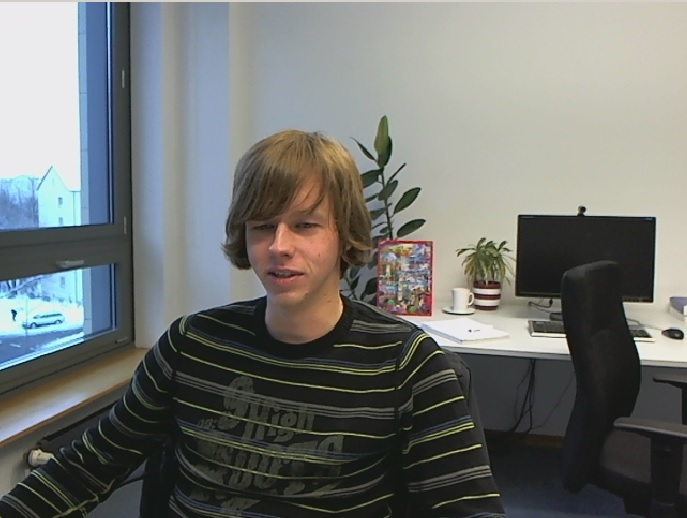
\includegraphics[scale=0.5]{PaulDefault120}
    \caption{A Frame in the input video}
    \label{fig:PaulDefault120}
%%encoded frame image
    
\includegraphics[scale=0.5]{PaulDefault120_91250kbps}
    \caption{Sample frame of fig \ref{fig:PaulDefault120} encoded at 250kbps}
    \label{fig:PaulDefaultencoded}
\end{figure} 

In a QP scale map, the darker regions in a frame indicate higher quantization. Even though quantization parameter used for encoding a block is closely related to the PSNR of the block, it is not the only determinative factor. The PSNR can also vary depending on the content. Generally, the lower frequency regions have better PSNR even when encoded with a higher QP. Also when a region of the frame is static, it tends to have better PSNR even when higher QP is used because of very less new information to be encoded. The PSNR map helps in visualizing the effect of movement of bits from non-ROI to ROI parts.

The image in Figure \ref{fig:PaulDefault120} shows a frame in the sample video conferencing content with resolution of 640x480 pixels and 30 frames per second. The image in figure \ref{fig:PaulDefaultencoded} shows the same frame when encoded with the codec configurations discussed in the previous section. The reason for considering a low bitrate of 250 kbps is that it will help in making the improvement in face region and decrease in quality of background more evident and hence will be useful in evaluating different algorithms. 

\begin{figure}[!h]
    \centering
    
\includegraphics[scale=0.5]{PaulDefault120_91250kbps_quant}
    \caption{Quantization map}
    \label{fig:PaulDefault120Quant}
    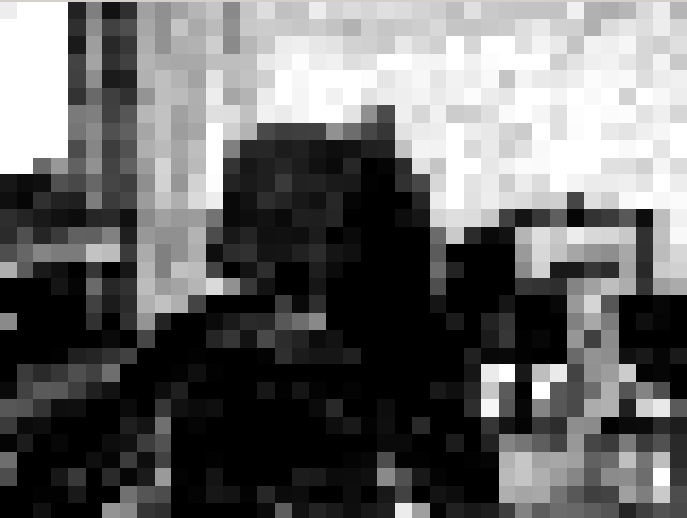
\includegraphics[scale=0.5]{PaulDefault120_91250kbps_psnr}
    \caption{Relative PSNR map}
    \label{fig:PaulDefault120PSNR}
\end{figure} 

The image in Figure \ref{fig:PaulDefault120Quant} shows the quant map of the frame in Figure \ref{fig:PaulDefaultencoded}. The darker regions in this map indicate usage of higher quantization parameter compared to the lighter regions. It can be noticed that since no information about region of interest is used while encoding the frame, the pattern of quantization appears almost random. The shape of the original content is almost not recognizable from the quantization map.

The image in Figure \ref{fig:PaulDefault120PSNR} shows the PSNR distribution for the frame in Figure \ref{fig:PaulDefaultencoded}. Similar to the quantization map, the lighter regions here represent the regions with higher PSNR, the darker regions indicate lower PSNR and worse quality. This map is relative within the frame and does not represent  absolute quality. This map is generated by considering the full range of PSNR of the image after removal of outliers. The map is generated by mapping the PSNR range between 10th percentile and 90th percentile of the whole frame to values between 0 to 255.

It is evident that the structure of the original content is preserved in the PSNR map. The background regions have better PSNR, the foreground has worse quality and the difference in quality is quite huge. The difference in the quality is due to the fact that background in a video conferencing scenario is mostly static and hence gets encoded better with every frame. On the other hand, the foreground has motion and new data to be encoded, hence it cannot achieve the same quality as the background. Since the focus of attention during video telephony is foreground or the face region, improving the face region must help in improving overall perceptual quality. The effect of such preferential encoding is studied in this work. The idea is to reduce the PSNR difference between foreground and background and to boost the quality of foreground (specifically face regions) to same level as background or even better.
%%
%%Bitrate Fluctuation and delay plots
%%
\subsubsection{Bitrate fluctuation - Delay plots}
The core idea in this work is to efficiently use the bits within the frame to encode the region of interest. The algorithms used to achieve that purpose should not alter the behavior of the codec in terms of frame level bit-consumption. As mentioned in previous sections, the encoder drops the frame in order to maintain strict VBV buffer compliance. The dropped frames result in jerky playback and hence should be avoided. The intelligent bit-allocation scheme should not contribute to more dropped frames.

The measured delay of every frame in the sequence is plotted to analyze bit-consumption behavior. A plot the delay of each frame is used to verify this. Figure \ref{fig:PaulDefault250kbpsDelay} is the delay plot of the bitstream encoded with 250 kbps (illustrated in Figure \ref{fig:PaulDefaultencoded}). Every point in the plot specifies the time taken by the corresponding frame (marked on the x-axis) to reach the decoder assuming zero transmission delay. The curve appears mostly smooth except for sudden drops (zero values). These zero-valued points indicate dropped frames. Since these frames are not included in the final bitstream and hence not transmitted, the delay is indicated as zero. 
\begin{figure}[!h]
    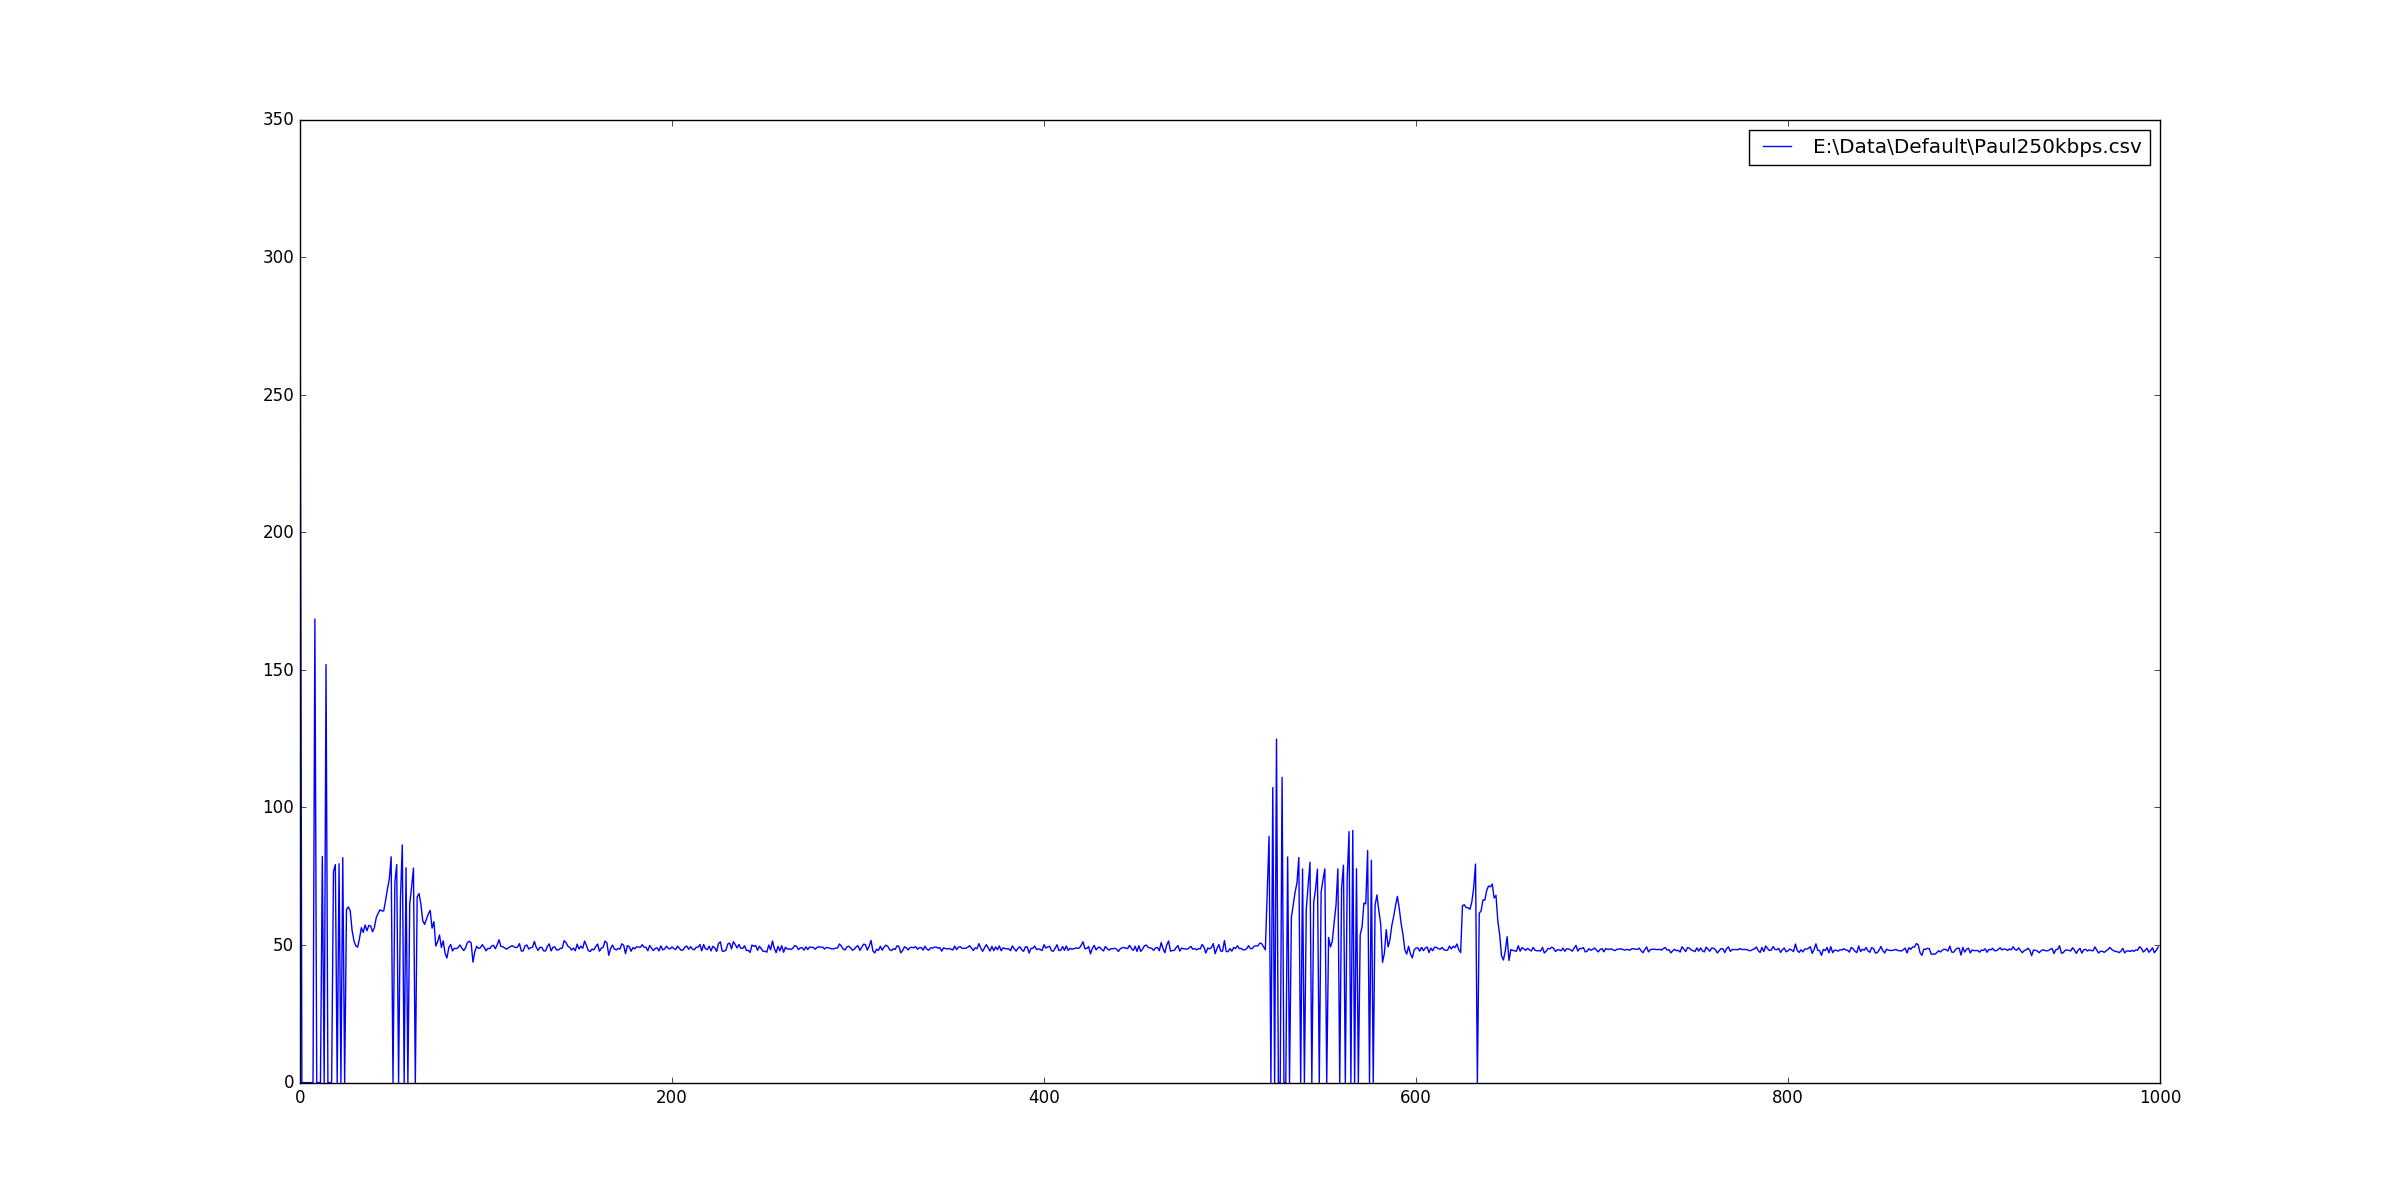
\includegraphics[scale=0.25]{PaulDefault250kbpsDelay}
    \caption{Delay plot}
    \label{fig:PaulDefault250kbpsDelay}
\end{figure} 
Ideally, an algorithm with intelligent bit allocation within a frame should not alter the shape of this graph. It is also desirable to not have any increase in the number of dropped frames. %Since, the algorithm is not expected to change overall behavior it is not expected to have reduction in number of dropped frames.
%
%Face Detection
%
\section{Face Detection}

Face detection algorithms are used to mark the region of interest in the current frame. All the algorithms considered for intelligent bit allocation involve improving the region of interest at the cost of rest of the frame. Therefore, it is very important to have high reliability with face detection. Any false detection will lead to degradation of the actual region of interest compared to normal encoding, this should be avoided in all scenarios. The damage caused by false detection is higher than the loss due to not detecting any face. Therefore, a high threshold must be used to declare any region of the frame as face.
\begin{figure}[!h]
    \centering
    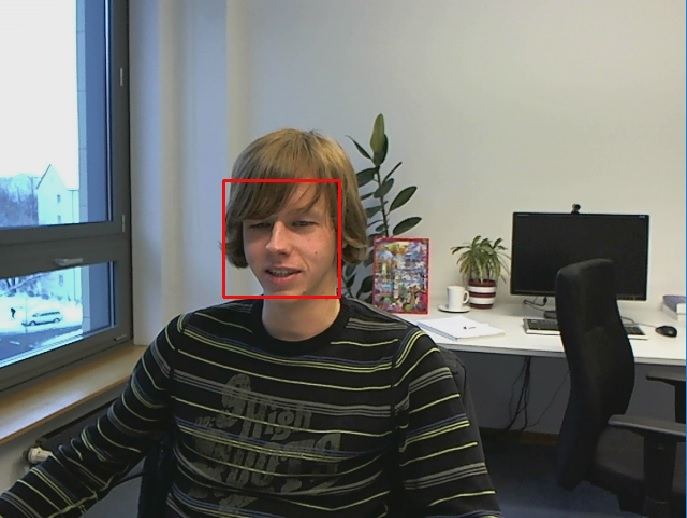
\includegraphics[scale=0.4]{PaulDefault120FaceRecognized}
    
\includegraphics[scale=0.4]{PaulDefault120FaceMap}
    \caption{Face Detection binary map}
    \label{fig:PaulDefault120FaceMap}
\end{figure}

 The face detection module itself shall not be a part of the encoder, but the output from the face detection is a binary file with face regions marked is used as input by the encoder. In this work, the face detection module uses input YUV to the encoder and marks the region of interest at the macro block level. Each byte value in the output file of face detection module represents a macro-block scanned in raster scan order. A value of 0xff signifies macro-block being part of the face or region of interest and 0x00 represents a normal macro-block. Figure \ref{fig:PaulDefault120FaceMap} represents the face map generated for the frame shown in Figure \ref{fig:PaulDefault120}. The region in white is considered as region of interest, this information is used inside the bitrate control module of the encoder to perform intelligent bit allocation.

Different approaches are used to detect the face region in the video. There is always a trade-off between accuracy of face detection algorithm and its complexity. The work presented here is mostly relevant to real time systems. Any added complexity due to additional module of face detection will cause significant delay which is totally unacceptable in such systems. Therefore, the algorithm chosen for face detection must be light weight and reasonably accurate in all lighting conditions. 

\subsection{Spatial Domain Face Detection}
In this approach, the face detection algorithms work directly on the pixel values. This approach is simple in terms of implementation. Many open-source solutions like OpenCV offers a ready to use solution that can be integrated with the codec library. It has large set of trained classifiers considering many types of faces and viewing angles. However, this is a computation intensive approach and almost impractical to use in the final solution. 
\subsection{Compressed domain Face Detection}
Most available face detection algorithms work on the pixel domain. These algorithms provide good level of detection accuracy. The main drawback of this approach is that they are computationally intensive. As discussed earlier, the use case considered in this work has very less room for additional computations. Therefore, in this work ways of compressed domain face detection is explored to detect faces with less computational requirements. 
Many works have been published
TBD LATER
%
%Different approaches
%
% 
\section{ROI based Intelligent Bitrate Control - Approaches}
There are many ways of using the additional information of knowing the region of interest. These methods should increase the quality of the ROI to gain maximum perceptual quality.
\subsection{QP offset}
The simplest and straight-forward way of creating a bias in quality for ROI and non-ROI is by using a QP offset between macroblocks belonging to these regions in the existing bitrate control module. The feedback from the encoder to rate control module will ensure that final bitrate is still met. A negative QP offset  is used for ROI regions, which triggers increase in QP of non-ROI regions due to the feedback. 

Such QP offsets will ensure the quality difference and shall not be overruled by bitrate control mechanisms. However, this approach might result in bitrate control over-reacting for the blocks around the ROI and encode them with extremely low quality. The magnitude of QP offset shall dictate the magnitude of shift in quality for the ROI. This approach is used to find right QP offset for best perceptual quality. 

It is perhaps a better idea to link the confidence quotient of face detection algorithms with the QP offset used. It should also be dependent on the area of the face, if the area of the ROI is considerably large in a video then the quality difference should be minimized. This is because there will be lesser non-ROI regions to compensate for additional bits used in ROI.
\begin{figure}[!h]
    \centering
    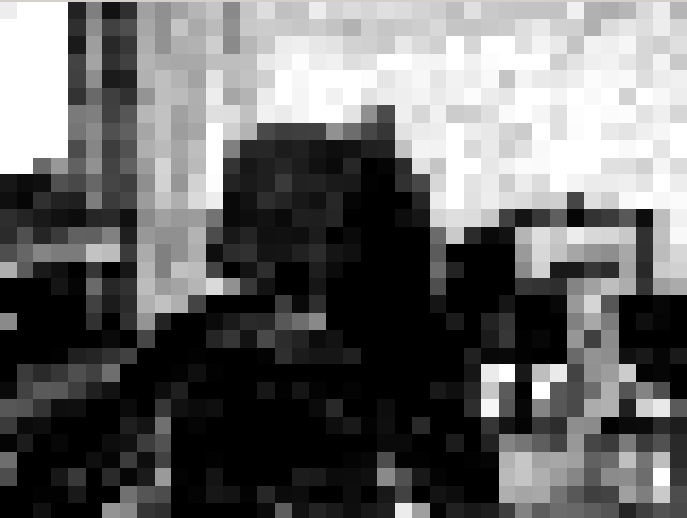
\includegraphics[scale=0.4]{PaulDefault120_91250kbps_psnr}
    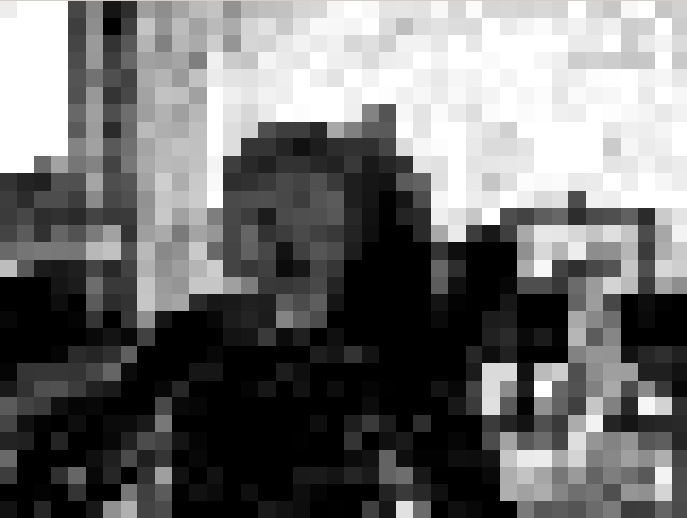
\includegraphics[scale=0.4]{QPOffset/paul120_250kbps_QPoffset4_psnr}
    
\includegraphics[scale=0.4]{PaulDefault120_91250kbps}
    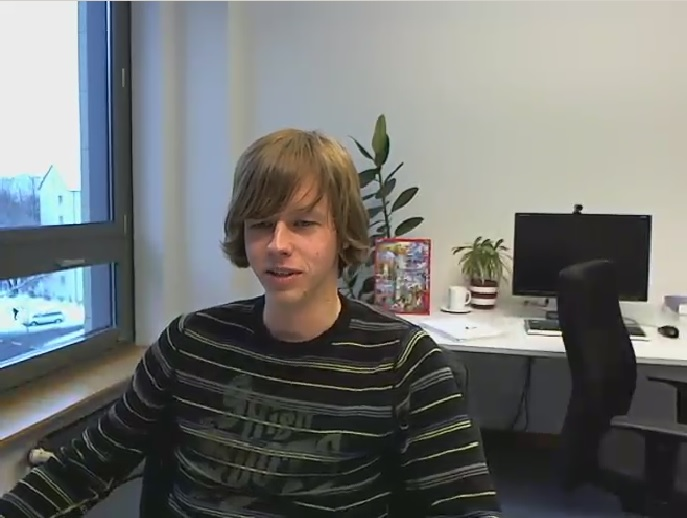
\includegraphics[scale=0.4]{QPOffset/paul120_250kbps_QPoffset4}
    
\includegraphics[scale=0.37]{PaulDefault120_91250kbps_quant}
    
\includegraphics[scale=0.4]{QPOffset/paul120_250kbps_QPoffset4_quant}    
    \caption{Comparing the images with QP offset of 4 for ROI}
    \label{fig:Default_QPOffsetCompare}
\end{figure}

\begin{figure}[!h]
    \centering
    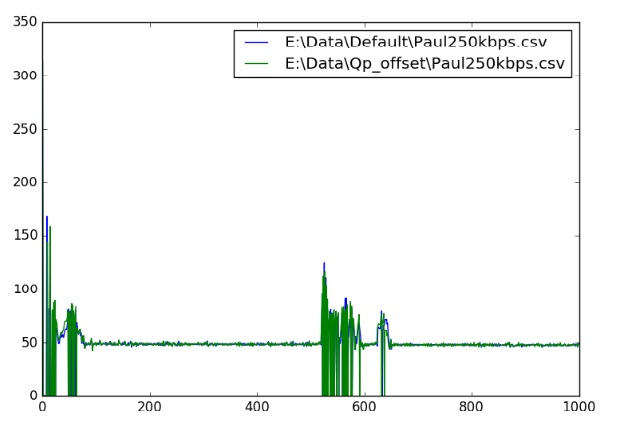
\includegraphics[scale=0.75]{QPOffset/Paul250kbps_QP_Offset_Delay}
    \caption{Delay Comparison of images with QP offset of 4 for ROI}
    \label{fig:DelayDefault_QPOffsetCompare}
\end{figure}

The images in \ref{fig:Default_QPOffsetCompare} shows the comparison between sample frame from original video with video encoded using QP offset of -4 for the ROI region and their corresponding attributes like PSNR map, Quant map. It can be seen that the QP in ROI region is considerably low compared to non ROI regions (marked with lighter shade of gray). The PSNR of the face is now more closer to the background region. The face appears much sharper due to additional boost in quality. The overall bitrate of the streams remained almost the same, the difference in the result is only due to the movement of bits. The number of dropped or skip frames were found to be same as original video. Figure \ref{fig:DelayDefault_QPOffsetCompare} shows the comparison of delay of original bitstream with the bitstream with QP offset for ROI. It can be seen that the delay behavior does not change significantly with skip/dropped frames at same locations.

The results of ROI based PSNR is tabulated in Table \ref{AllPSNR1}. It can be noticed that the ROI PSNR now approaches the overall frame PSNR. This difference can be further altered by tuning the QP offset used.
\begin{table} [h!]
\centering
\begin{tabular}{ |c|c|c|c| }
 \hline
Methodology & Content & PSNR Avg (dB) & PSNR ROI (dB) \\
 \hline 
QP Offset & Paul640x480, 250kbps & 38.90 & 38.88 \\ 
 & Johny1280x720 750kbps & 40.49 & 40.22 \\  
 \hline
Reaction Factor & Paul640x480, 250kbps & 38.22 & 39.50 \\ 
 & Johny1280x720 750kbps & 39.71 & 40.74 \\  
 \hline
\end{tabular}
 \caption{PSNR Comparison for different approaches}
 \label{AllPSNR1}
\end{table}

%
\subsubsection{Tuning QP Offset}
As mentioned earlier, the methods discussed in this work only aim to re-distribute the bits within a frame based on the region of interest. The extent of re-distribution should be carefully chosen to avoid degradation of the background to an extent that artifacts become noticeable to the viewer even though they are not expected to concentrate on those regions. Ideal level of redistribution will make sure that there is maximum transfer of bits from non-ROI region to ROI without creating any visible artifacts in the image.
\begin{figure}[!h]
    \centering
    
\includegraphics[scale=0.43]{QPOffset/trialOffset/Paul250kbps_offset2}
    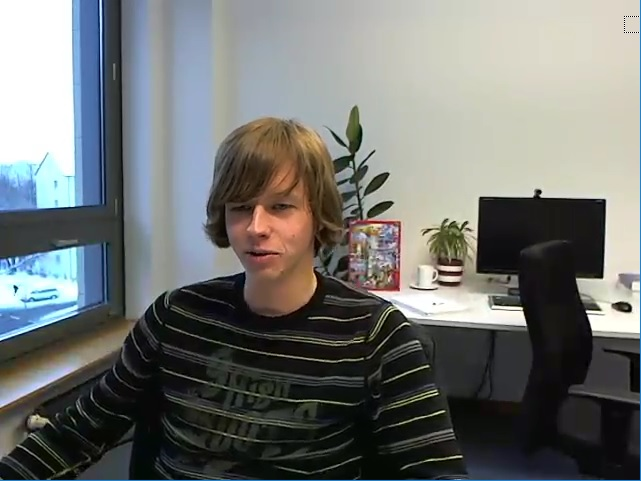
\includegraphics[scale=0.43]{QPOffset/trialOffset/Paul250kbps_offset4}
    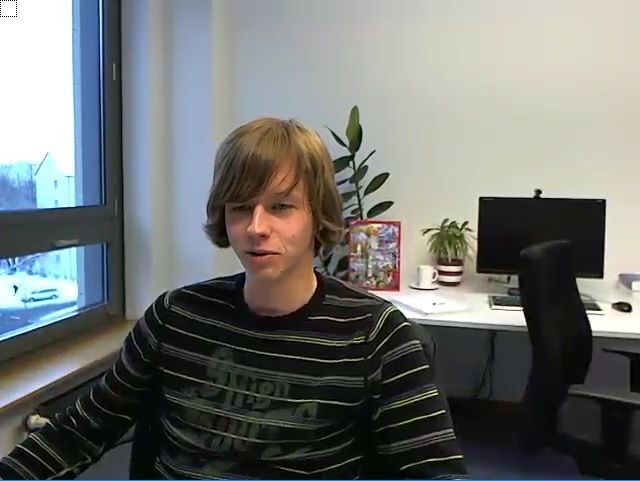
\includegraphics[scale=0.43]{QPOffset/trialOffset/Paul250kbps_offset6}
    
\includegraphics[scale=0.43]{QPOffset/trialOffset/Paul250kbps_offset8}  
    \caption{Tuning QP offset - Trial QP offsets used are 2, 4, 6 and 8 in raster scan order}
    \label{fig:Default_QPOffsetTuning}
\end{figure}
\begin{figure}[!h]
    \centering
    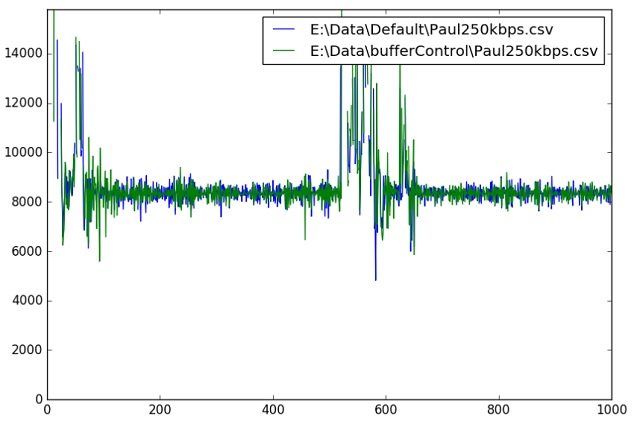
\includegraphics[scale=0.75]{BufferControl/Paul250kbps_Buffer_Control_Delay}
    \caption{Delay Comparison of original video with ROI based reaction factor modification}
    \label{fig:DelayDefault_BufferControltCompare}
\end{figure}

In this work, various offsets were used to study the effect of magnitude of QP offset on perceptual quality. The results shown in Figure \ref{fig:Default_QPOffsetTuning} shows that, as QP offset increases the face region appears more sharper which improves the overall perceptual quality of the frame. The image with QP offset of 8 appears to not have any noticeable blockiness in the background. However, using a very high QP offset triggers another problems that is not shown in the sample images. Due to increased QP offset, the encoder is forced to use lower QP even when virtual buffer is critically full. This increases the number of skipped/dropped frames in the entires sequence. The sample video consisted of 1000 frames and a total of 44, 46, 46 and 50 frames were dropped in the sequence with QP offset of 2, 4, 6 and 8 respectively. This increase in skip frames reduces the smoothness of the playback which is annoying to the viewer. Therefore, the increase in QP offset should tuned not only considering the degradation of the background quality but also by assessing any other side effects like increase in dropped frames.
%
%Discuss the impact of ratio of ROI mbs to non-ROI mb's
\subsubsection{Area of Region of Interest}
The variation in QP offset discussed in the above section correspond to same sequence where the ratio of number of ROI macroblocks to number of non-ROI macroblocks is almost same. In the sample sequence used, 46 to 50 macroblocks out of 1200 total macroblocks belong to face (ROI). Therefore, the ROI is less than 5 percent of the entire video frame. This is comparatively smaller ROI, it is possible to use very high QP offsets since there are large number of non-ROI frames to compensate for the consumption of bits at ROI. However, based on the focal length of the camera and distance from camera, the area of face in video conference can change considerably. For instance, when the area of ROI is half of the entire frame, usage of higher QP offsets will cause severe degradation in the quality of non-ROI macroblocks. In order severe degradation of the background, the magnitude of the QP offset should be inversely proportional to the ratio of ROI to non-ROI.

The algorithm implemented to use area of ROI, calculates the QP offset using linear relationship described in equation \ref{Eq:QP_offset}
\begin{equation}
	\label{Eq:QP_offset}
	\begin{aligned}
	dq_{roi} = -round\Big(\frac{M}{M_{roi} * 3}\Big) \\
	dq_{roi} = clip(dq_{roi}, -1 , -6)
	\end{aligned}	
\end{equation}
where, $dq_{roi}$ is the offset of used for ROI blocks, $M$ is the total number of macroblocks in the frame, $M_{roi}$ is the total number of macroblocks marked as region-of-interest. The negative sign in the equation implies the calculated offset is negative, which results is QP lower non-ROI blocks. 

It is evident from equation \ref{Eq:QP_offset}, there is no QP offset for ROI region if ROI region covers more than two-third of the whole frame. Subsequently, the offset increases linearly with increase in ROI area. A offset is clipped between -1 to -6 to avoid extreme offsets.

The QP offsets calculated so far is only applied to ROI region. The bitrate control module is help responsible to increase QP of the non-ROI. The over-consumption of bits in ROI triggers the reaction by Bitrate control to increase the QP for non-ROI blocks. However, this approach of one-sided offset results in the artifact event in figure TBD. It can be noticed the the blocks above ROI belonging to non-ROI generally have lower QP compared to non-ROI blocks below the face region. This is because, the QP of the non-ROI blocks is increased by bitrate control module only after it sees the over-consumption after encoding the ROI blocks. This results in usage of average QP for non-ROI blocks before encoding ROI. Once the ROI is encoded with lower QP, the bits over-consumption is compensated for by increasing the QP of non-ROI blocks encoded after ROI blocks.

A two sided QP offset is used to avoid the behavior described above. The non-ROI blocks are assigned with positive QP offset, which can compensate the over-consumption in ROI blocks. Since the non-ROI blocks from start of the frame are encoded with higher QP, there will be surplus of bits already which can be used in encoding ROI blocks. In ideal scenario, the negative and positive QP offsets must negate each others effect resulting in frame level bits being unchanged had the frame been encoded without any offset.

The study in \cite{ROI-Coding-paper} suggests that, for frame level bitcount to be constant, the average QP of the frame must remain unchanged before and after adding the offsets. This is an observation made after multiple experiments. The equation \ref{Eq:QP_offset_double} shows computing the offset for non-ROI based on offset calculated for non-ROI in eq \ref{Eq:QP_offset}
\begin{equation}
	\label{Eq:QP_offset_double}
		dq_{non-roi} = \frac{M_{roi} * dq_{roi}}{M - M_{roi}}
\end{equation}
where, $dq_{non-roi}$ is a positive QP offset used for non-ROI blocks when negative QP offset of $dq_{roi}$ is used for ROI blocks. 
\subsection{Reaction Factor - Buffer control} 

\begin{figure}[!h]
    \centering
    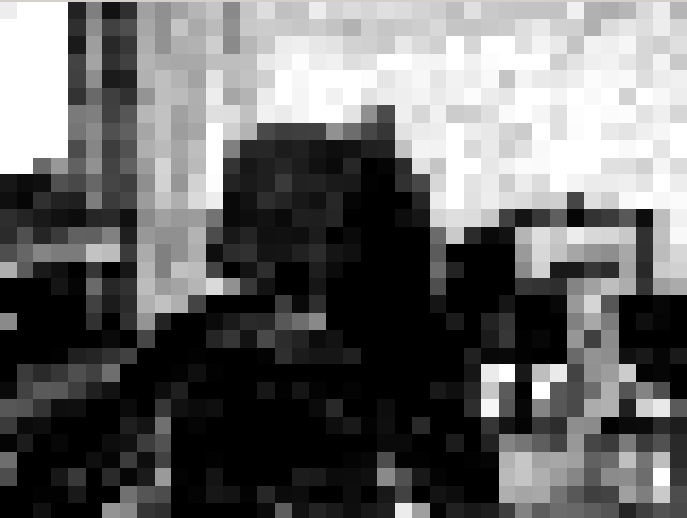
\includegraphics[scale=0.4]{PaulDefault120_91250kbps_psnr}
    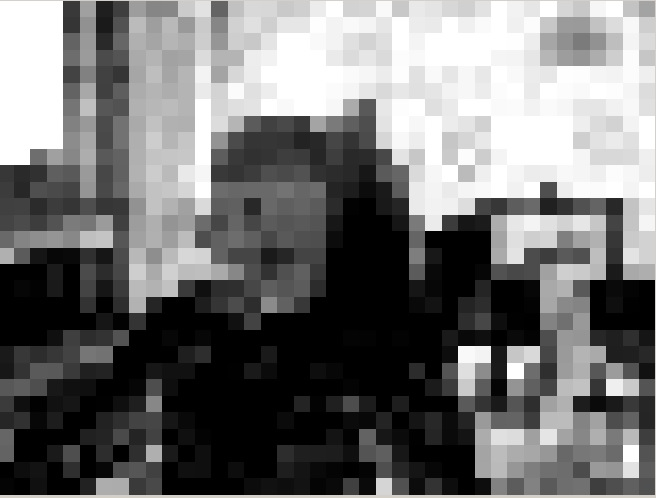
\includegraphics[scale=0.4]{BufferControl/paul120_250kbps_BufferControl_psnr}
    
\includegraphics[scale=0.4]{PaulDefault120_91250kbps}
    
\includegraphics[scale=0.4]{BufferControl/paul120_250kbps_bufferControl}
    
\includegraphics[scale=0.37]{PaulDefault120_91250kbps_quant}
    
\includegraphics[scale=0.4]{BufferControl/paul120_250kbps_BufferControl_quant}    
    \caption{Comparing the images with modified reaction for ROI macroblcoks}
    \label{fig:Default_BufferControlCompare}
\end{figure}

The second approach of using the ROI information to enhance quality of ROI is by using different buffer controls inside the bitrate control module. The bitrate control module used in this study compensates for the overconsumption or underconsumption of bits in the past by adjusting the delta bits during bit allocation of the future frames. This corrected allocation happens at every macroblock level. For instance, if there is excessive consumption of bits in the past macro-blocks, the excess is subtracted from bit budget of certain number of future frames known as reaction factor. If the reaction factor is low, the excess or shortage of bits is shared by a large number of macro-blocks.

The reaction factor is used to allocate additional bits to ROI by using different reaction factors for macro-blocks belonging to the ROI. For instance, in case of underconsumption in the past, the excess bits available for future macroblocks is forced to be used aggressively for macroblocks belonging to ROI. On the other hand whenever there is overconsumption in the past, the bits are reduced more aggressively for macroblocks belonging to non-ROI. The advantage of this approach over QP offset approach is that the bit-allocation is still controlled within the rate control module and its decisions are not overridden by external offsets. This guarantees better buffer compliance. The results shown in Figure \ref{fig:Default_BufferControlCompare} compares the output with modified reaction factor based on region of interest and original video. It can be noticed that PSNR of the face regions is very close to that of the background. The data in Table \ref{AllPSNR1} shows that PSNR of ROI region is actually higher than the overall frame PSNR. The delay plots in \ref{fig:DelayDefault_BufferControltCompare} shows there is no significant changes in the delay or bitrate consumption.
%
%
%Bibiliography and reference
%
%
%
\clearpage
\begin{thebibliography}{9}
\bibitem{HighQualityROICodingForVideoConferencing} 
Manzur Murshed and James Brown. 
\textit{High Quality Region-of-Interest Coding for Video Conferencing based Remote General Practitioner Training}. 
The Fifth International Conference on eHealth, Telemedicine, and Social Medicine.

\bibitem{ComparingCodingEfficiency} 
J. Ohm. G. J. Sullivan, H. Schwarz, Thiow Keng Tan and T. Wiegand.
\textit{Comparison of the Coding Efficiency of Video Coding Standards—Including High Efficiency Video Coding (HEVC).}
 IEEE Transactions on Circuits and Systems for Video Technology ( Volume: 22, Issue: 12, Dec. 2012 )

\bibitem{JVTF086}
Siwei Ma, Wen Gao, Yan Lu and Hanqing Lu.
\textit{Proposed draft description of rate control on JVT standard. }
Joint Video Team (JVT) of ISO/IEC MPEG and ITU-T VCEG (ISO/IEC JTC1/SC29/WG11 and ITU-T SG16 Q.6) 6h Meeting: Awaji, 5-13, December, 2002.

\bibitem{ROI-Coding-paper}
Manzur Murshed, Md. Atiur Rahman Siddique, Saikat Islam and James Brown.
\textit{High Quality Region-of-Interest Coding for Video Conferencing based Remote General Practitioner Training.}
eTELEMED 2013 : The Fifth International Conference on eHealth, Telemedicine, and Social Medicine

\bibitem{ROI-background-blurring}
A. Cavallaro, O. Steiger, T. Ebrahimi, \textit{"Semantic video analysis for adaptive content delivery and automatic description"}
IEEE Trans. Circuits Syst. Video Technol., vol. 15, no. 10, pp. 1200-1209, Oct. 2005.

\bibitem{Perception-model-of-face}
Mai Xu, Xin Deng, Shengxi Li, \textit{"Region-of-Interest Based Conversational HEVC Coding with Hierarchical Perception Model of Face"}
IEEE Journal of Selected Topics in Signal Processing ( Volume: 8, Issue: 3, June 2014 )

\bibitem{ROI-bit-allocation-h264}
G.-L. Wu, Y.-J. Fu, S.-Y. Chien, \textit{"Region-based perceptual quality regulable bit allocation and rate control for video coding applications"},
Proc. VCIP, 2012.

\bibitem{pre-postprocessig-ROI-codec-independent}
Holger Meuel, Florian Kluger, Jorn Ostermann, \textit{"Codec independent region of interest video coding using a joint pre- and postprocessing framework"}, 
IEEE International Conference on Multimedia and Expo (ICME), July 2016

\bibitem{ROI-MV-based-face-tracking}
Lin Tong, K.R. Rao \textit{"Region of interest based H.263 compatible codec and its rate control for low bit rate video conferencing"}, 
Intelligent Signal Processing and Communication Systems, 2005. ISPACS 2005. Proceedings of 2005 International Symposium on, vol., no., pp. 249- 252, 13-16 Dec. 2005.

\bibitem{InTech-Rate-control-in-video-coding}
Zongze Wu, Shengli Xie1, Kexin Zhang and Rong Wu, \textit{"Rate Control in Video Coding"},
Recent Advances on Video Coding, J. Del Ser Lorente, Ed. InTech,
2011, 79–117. \url{http://www.intechopen.com/books/recent-advances-onvideo-coding/rate-control-in-video-coding}

\bibitem{ROI-aerial-surveillance}
Holger Meuel, Marco Munderloh, Jörn Ostermann, \textit{"Low Bit Rate ROI Based Video Coding for HDTV Aerial Surveillance Video Sequences"}, 
Proc. of the IEEE Conf. on Computer Vision and Pattern Recognition - Workshops (CVPRW), pp. 13-20, June 2011.

\bibitem{foveated-rate-control}
S. Lee, A. C. Bovik, \textit{"Fast algorithms for foveated video processing"},
IEEE Trans. Circuits Syst. Video Technol., vol. 13, no. 2, pp. 149-161, Feb. 2003.

\bibitem{ROI-rate-control-H264}
Fan Li, Na Li, \textit{"Region-of-interest based rate control algorithm for H.264/
AVC video coding"},
Multimed Tools Appl (2016) 75:4163–4186
 
%%Not so Important Reference
\bibitem{human-vision-proof-NSI}
B. Wandell, \textit{"Foundations of Vision"}, 1995, Sinauer.

\bibitem{Leaky-bucket-NSI}
\url{http://www.eenadupratibha.net/pratibha/engineering/content_three_tra_layer_u6.html}
\end{thebibliography}
\end{document}